\documentclass[a4paper]{article}
\usepackage{amsfonts}
\usepackage{amsmath}
\usepackage{amssymb}
\usepackage{graphicx}     

\begin{document}
  
\noindent \large Auteur: Rubin Cuypers \\
\noindent \large Studierichting: Informatica\\
\noindent \large Oefeningenreeks 5D nr. 5.1\\

\medskip

\normalsize

$y^2=2x-1$ en $y=2x-3$\\

$x_1=\dfrac{y^2+1}{2}$ en $ x_2=\dfrac{y+3}{2}$\\

$\Rightarrow S=\displaystyle \int_{-1}^2 \left( \dfrac{y+3}{2} -\dfrac{y^2+1}{2}\right)dy$\\

$=\displaystyle \int_{-1}^2 \dfrac{1}{2} \left(-y^2+y+2\right) dy$\\

$=\left[-\dfrac{y^3}{6} +\dfrac{y^2}{4} + y \right]_{-1}^2$\\

$=-\dfrac{4}{3} + 1 + 2 - \left(\dfrac{1}{6} + \dfrac{1}{4} -1\right)$\\

$ = \dfrac{27}{12}$\\

$ = \dfrac{9}{4}$\\

\begin{figure}[h]
\centering
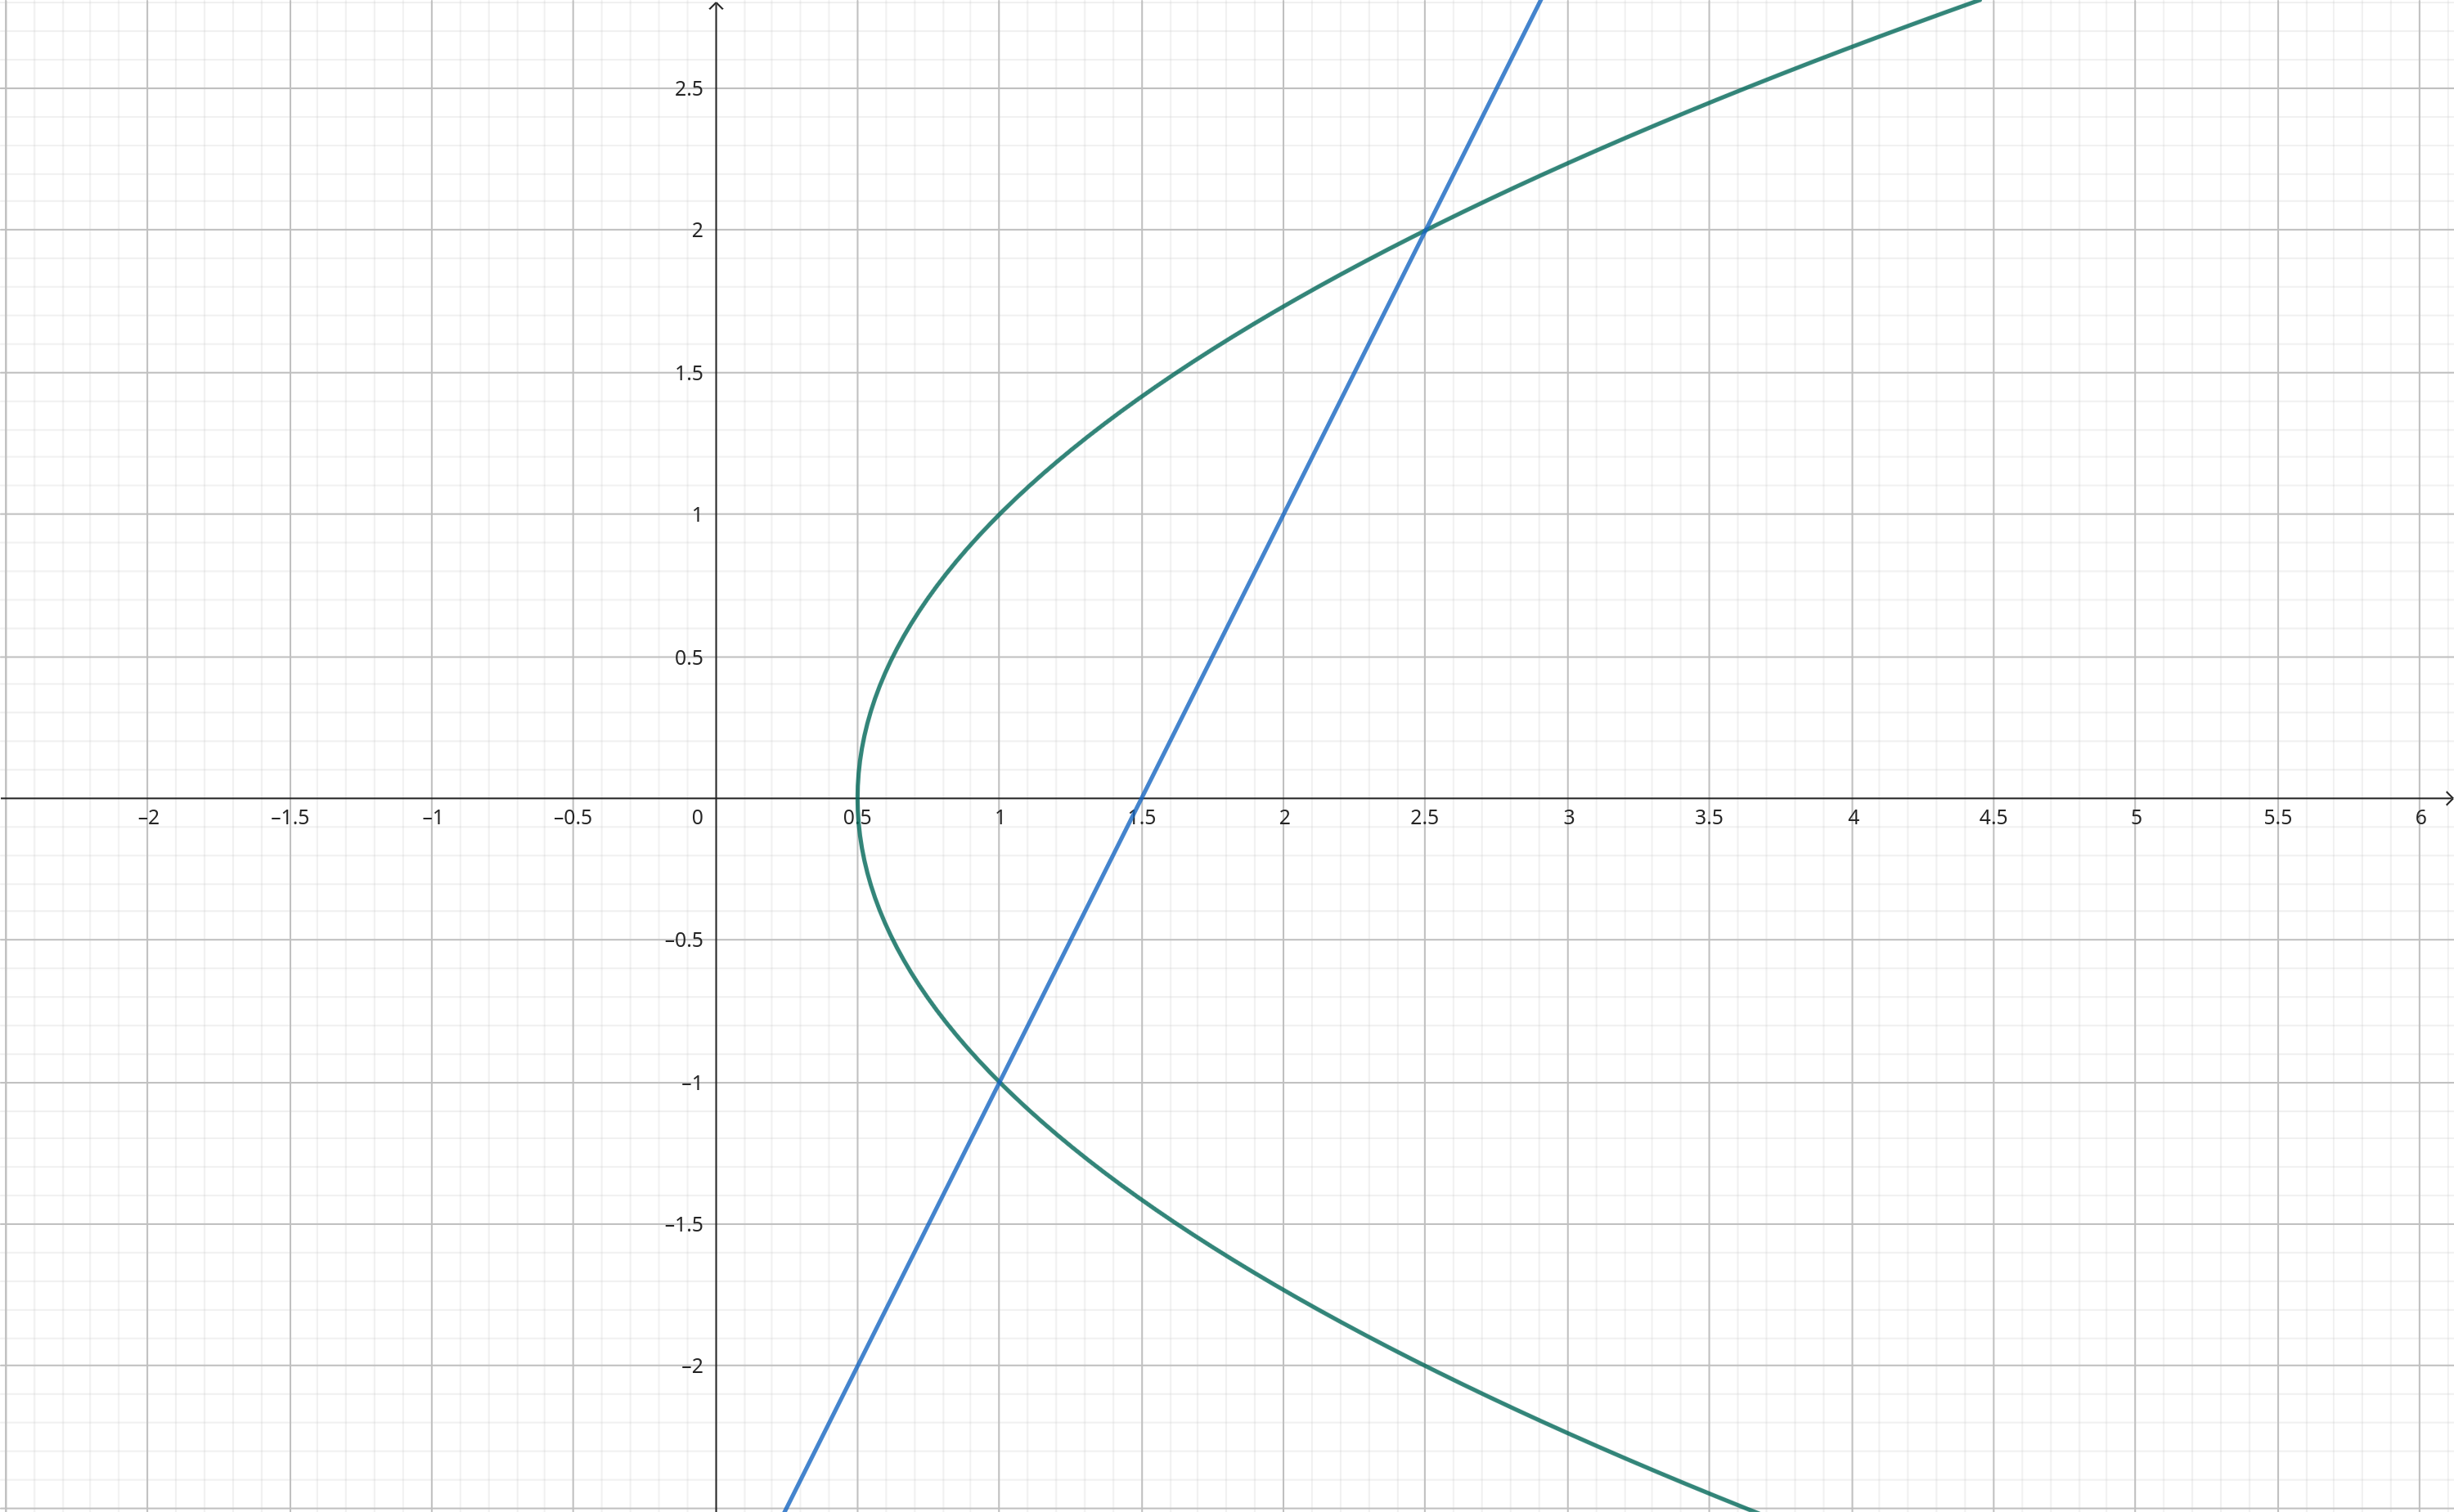
\includegraphics[width=\linewidth]{5D-5.1-rubin.cuypers.INF.png}\\
\end{figure}


\begin{thebibliography}{999}
%\bibitem{a} Referentie
\end{thebibliography}
\end{document} 
